\documentclass[11pt,a4paper]{article}

\usepackage[margin=1in]{geometry}
\usepackage[T1]{fontenc}
\usepackage[utf8]{inputenc}
\usepackage{lmodern}
\usepackage{amsmath,amssymb,amsfonts,mathtools,bm}
\usepackage{booktabs,longtable,array,tabularx}
\usepackage{enumitem}
\usepackage{xcolor}
\usepackage{hyperref}
\usepackage{listings}
\usepackage{tikz}
\usetikzlibrary{arrows.meta,positioning}

\hypersetup{
  colorlinks=true,
  linkcolor=blue!60!black,
  urlcolor=blue!60!black
}

\lstset{
  basicstyle=\ttfamily\small,
  breaklines=true,
  columns=fullflexible,
  keepspaces=true,
  frame=single
}

\newcommand{\R}{\mathbb{R}}
\newcommand{\vect}[1]{\bm{#1}}
\newcommand{\mat}[1]{\bm{#1}}
\newcommand{\trans}{^{\mathsf T}}
\newcommand{\code}[1]{\texttt{#1}}

\title{\textbf{Quadruped-Control-OCS2-ROS2}\\A Detailed Mathematical and Architectural Report}
\author{Generated from direct workspace inspection}
\date{March 9, 2026}

\begin{document}
\maketitle
\tableofcontents
\clearpage

\section{Scope and Reading Strategy}
This report covers the workspace rooted at \code{/home/kaan/quad\_ocs2\_ws}, with emphasis on the project-specific stack under \code{src/Quadruped-Control-OCS2-ROS2}. The workspace is not a single package: it is a ROS 2 meta-workspace that vendors a large portion of OCS2, Pinocchio, hpp-fcl, MuJoCo assets, plane segmentation utilities, and several robotic example packages. The custom quadruped application logic is concentrated in five packages:
\begin{itemize}[leftmargin=*]
\item \code{motion_control}: SQP-MPC, reference management, whole-body control, constraints, and state estimation.
\item \code{mujoco_simulator}: MuJoCo-based simulation, rendering, and ROS 2 I/O.
\item \code{user_command}: terminal-driven gait and goal command publication.
\item \code{launch_simulation}: launch orchestration.
\item \code{legged_msgs}: custom ROS 2 messages and services connecting the stack.
\end{itemize}

The remainder of the workspace mainly supplies mathematical infrastructure, kinematics/dynamics libraries, optimization backends, and examples reused by the custom stack.

\section{Executive Summary}
At a system level, this workspace implements a centroidal-model nonlinear MPC controller for quadrupeds, wrapped in ROS 2 and closed in simulation through MuJoCo. The control chain is
\begin{equation}
\text{user command} \rightarrow \text{reference manager} \rightarrow \text{SQP-MPC} \rightarrow \text{WBC QP} \rightarrow \text{joint command} \rightarrow \text{MuJoCo},
\end{equation}
with sensor/state feedback returning from MuJoCo to the controller.

For the default B1 configuration inspected here, the project uses:
\begin{itemize}[leftmargin=*]
\item a \emph{full centroidal} model (\code{centroidalModelType = 0}),
\item a 24-dimensional OCS2 state,
\item a 24-dimensional OCS2 input,
\item a 40 Hz MPC update rate,
\item a 500 Hz whole-body-control update rate,
\item a 1 kHz MuJoCo integration step,
\item a weighted whole-body QP with 42 decision variables.
\end{itemize}

The project mathematically decomposes into three layers:
\begin{enumerate}[leftmargin=*]
\item a switched-mode optimal control problem on centroidal dynamics,
\item a whole-body inverse-dynamics QP that lifts centroidal commands into joint torques,
\item a linear contact-aided state estimator used when IMU mode is enabled.
\end{enumerate}

\section{Workspace Anatomy}
\subsection{Top-Level Decomposition}
The repository \code{src/Quadruped-Control-OCS2-ROS2} contains the following major subsystems:
\begin{itemize}[leftmargin=*]
\item \code{legged_control}: the custom quadruped application packages.
\item \code{ocs2_ros2}: vendored OCS2 packages, including \code{ocs2_core}, \code{ocs2_mpc}, \code{ocs2_sqp}, \code{ocs2_centroidal_model}, and many examples.
\item \code{pinocchio}: rigid-body kinematics and dynamics.
\item \code{hpp-fcl}: collision geometry utilities.
\item \code{qpOASES-master}: QP solver used by the whole-body controller.
\item \code{mujoco}: MuJoCo binaries and models.
\item \code{plane_segmentation_ros2}: terrain/perception utilities vendored from related OCS2 ecosystems.
\item \code{ocs2_robotic_assets}: robot asset package used by OCS2 examples.
\end{itemize}

\subsection{Custom Package Roles}
\begin{table}[ht]
\centering
\small
\begin{tabularx}{\textwidth}{>{\ttfamily}l >{\raggedright\arraybackslash}X >{\raggedright\arraybackslash}X}
\toprule
Package & Runtime role & Key artifacts \\
\midrule
motion\_control & Core controller package. Builds the motion-control library and the \code{legged\_robot\_sqp\_mpc} node. & LeggedRobotInterface, MPC\_WBC\_ROS\_Interface, WeightedWbc, KalmanFilterEstimate, gait/reference managers, constraints \\
mujoco\_simulator & Simulation, visualization, actuator model, contact detection, state/sensor publication & MujocoSimulation, SimulatorNode, robot XML/URDF model folders \\
user\_command & Keyboard-driven operator interface for gait switching and target trajectory commands & GaitKeyboardPublisher, TargetTrajectoriesKeyboardPublisher, UserCommandNode \\
launch\_simulation & Launch-time parameter plumbing and node orchestration & \code{legged\_robot\_sqp.launch.py} \\
legged\_msgs & Wire protocol between simulator, controller, and user-command nodes & state/sensor/control messages and the \code{StartControl} service \\
\bottomrule
\end{tabularx}
\end{table}

\subsection{Supported Robot Configurations}
The workspace includes multiple model/config folders:
\begin{itemize}[leftmargin=*]
\item \code{a1}
\item \code{a1\_custom}
\item \code{b1}
\item \code{b1\_custom}
\item \code{quad\_mini}
\end{itemize}
The default launch argument in \code{launch\_simulation/launch/legged\_robot\_sqp.launch.py} is \code{robot\_type:=b1}. Therefore, most numerical values quoted in this report are taken from the inspected B1 configuration.

\section{End-to-End Runtime Architecture}
\subsection{Control Graph}
\begin{figure}[ht]
\centering
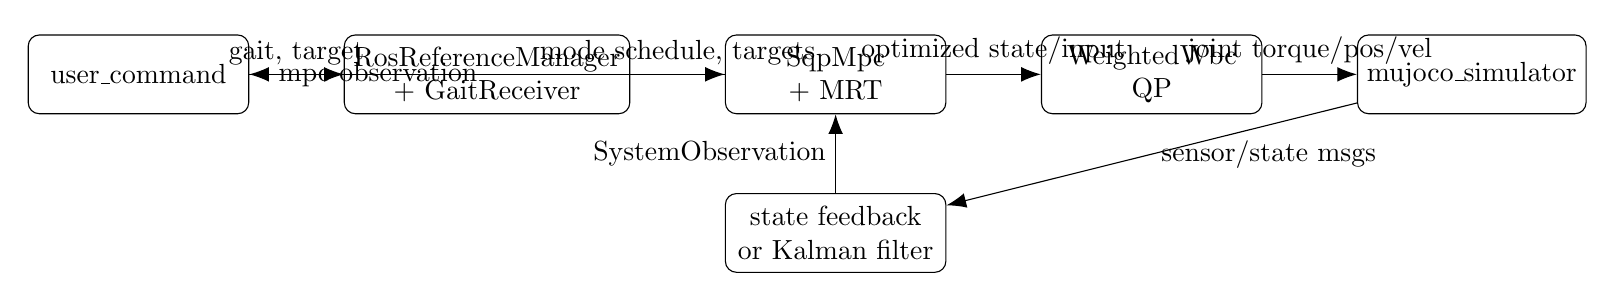
\begin{tikzpicture}[
  node distance=10mm and 12mm,
  box/.style={draw, rounded corners, align=center, minimum width=28mm, minimum height=10mm},
  line/.style={-{Latex[length=2.5mm]}}
]
\node[box] (user) {user\_command};
\node[box, right=of user] (ref) {RosReferenceManager\\+ GaitReceiver};
\node[box, right=of ref] (mpc) {SqpMpc\\+ MRT};
\node[box, right=of mpc] (wbc) {WeightedWbc\\QP};
\node[box, right=of wbc] (sim) {mujoco\_simulator};
\node[box, below=of mpc] (est) {state feedback\\or Kalman filter};

\draw[line] (user) -- node[above] {gait, target} (ref);
\draw[line] (ref) -- node[above] {mode schedule, targets} (mpc);
\draw[line] (mpc) -- node[above] {optimized state/input} (wbc);
\draw[line] (wbc) -- node[above] {joint torque/pos/vel} (sim);
\draw[line] (sim) -- node[right] {sensor/state msgs} (est);
\draw[line] (est) -- node[left] {SystemObservation} (mpc);
\draw[line] (mpc) -- node[left] {mpc observation} (user);
\end{tikzpicture}
\caption{Closed-loop data path in the custom stack.}
\end{figure}

\subsection{ROS 2 Topics and Services}
\begin{table}[ht]
\centering
\small
\begin{tabularx}{\textwidth}{>{\ttfamily}l >{\ttfamily}l >{\raggedright\arraybackslash}X}
\toprule
Name & Type & Role \\
\midrule
joint\_control\_data & topic & WBC output consumed by MuJoCo simulator \\
simulator\_state\_data & topic & ground-truth state feedback from MuJoCo \\
simulator\_sensor\_data & topic & IMU + joint + contact sensor stream for state estimation \\
legged\_robot\_mpc\_observation & topic & current observation published by motion\_control \\
legged\_robot\_mpc\_target & topic & target trajectory updates from user\_command to motion\_control \\
legged\_robot\_mpc\_mode\_schedule & topic & gait template updates from user\_command to GaitReceiver \\
start\_control & service & one-shot handshake returning the simulator's initial state \\
\bottomrule
\end{tabularx}
\end{table}

\subsection{Launch Sequence}
The launch file does the following:
\begin{enumerate}[leftmargin=*]
\item resolves model/config file paths from the selected \code{robot\_type},
\item starts \code{mujoco\_simulator},
\item starts \code{user\_command},
\item waits 2 seconds,
\item starts \code{motion\_control}'s \code{legged\_robot\_sqp\_mpc} node.
\end{enumerate}
Both simulator and user-command nodes are launched with a \code{gnome-terminal --} prefix, which is convenient on desktop Ubuntu but makes the launch setup less portable in headless or containerized environments.

\section{Internal Mathematical Model}
\subsection{State, Input, and Contact Mode}
For the default 12-actuated-DOF quadruped, the OCS2 state used by \code{motion\_control} is
\begin{equation}
\vect{x} =
\begin{bmatrix}
\vect{v}_{\mathrm{com}} \\
\vect{k}/m \\
\vect{p}_b \\
\vect{\theta}_{zyx} \\
\vect{q}_j
\end{bmatrix}
\in \R^{24},
\end{equation}
where
\begin{itemize}[leftmargin=*]
\item $\vect{v}_{\mathrm{com}} \in \R^3$ is normalized linear centroidal momentum, numerically stored as center-of-mass velocity,
\item $\vect{k}/m \in \R^3$ is normalized angular centroidal momentum,
\item $\vect{p}_b \in \R^3$ is base position,
\item $\vect{\theta}_{zyx} \in \R^3$ is base orientation in ZYX Euler angles,
\item $\vect{q}_j \in \R^{12}$ is the joint-position vector.
\end{itemize}

The control input is
\begin{equation}
\vect{u} =
\begin{bmatrix}
\vect{f}_{LF} \\
\vect{f}_{RF} \\
\vect{f}_{LH} \\
\vect{f}_{RH} \\
\dot{\vect{q}}_j
\end{bmatrix}
\in \R^{24},
\end{equation}
with four 3D contact-force vectors and 12 joint velocities.

The contact mode is encoded as a 4-bit integer
\begin{equation}
\sigma = 8 c_{LF} + 4 c_{RF} + 2 c_{LH} + c_{RH}, \qquad c_{\ell}\in\{0,1\},
\end{equation}
which exactly matches the implementation of \code{stanceLeg2ModeNumber()} in \code{MotionPhaseDefinition.h}. Thus $\sigma \in \{0,\dots,15\}$ spans every stance/swing pattern of the four feet.

\subsection{Centroidal Dynamics Layer}
The project selects \code{centroidalModelType = 0}, i.e. full centroidal dynamics. The implementation delegates the actual flow map to OCS2/Pinocchio through \code{LeggedRobotDynamicsAD}, which wraps \code{PinocchioCentroidalDynamicsAd}. At a modeling level, the continuous-time structure is
\begin{equation}
\dot{\vect{x}} = \vect{f}(\vect{x},\vect{u}; \mathcal{M}),
\end{equation}
with $\mathcal{M}$ the rigid-body model extracted from the robot URDF.

The centroidal momentum rate follows the familiar structure
\begin{equation}
\dot{\vect{h}} =
\sum_{i \in \mathcal{C}(\sigma)}
\begin{bmatrix}
\vect{f}_i \\
(\vect{r}_i - \vect{c}) \times \vect{f}_i
\end{bmatrix}
+
\begin{bmatrix}
m \vect{g} \\
\vect{0}
\end{bmatrix},
\end{equation}
where $\vect{c}$ is the center of mass, $\vect{r}_i$ are contact locations, and $\mathcal{C}(\sigma)$ is the active contact set implied by the mode.

The remaining state coordinates evolve through the centroidal-to-rigid-body mapping:
\begin{equation}
\dot{\vect{p}}_b = \vect{v}_b, \qquad
\dot{\vect{\theta}}_{zyx} = \mat{T}(\vect{\theta}_{zyx}) \vect{\omega}_b, \qquad
\dot{\vect{q}}_j = \dot{\vect{q}}_j,
\end{equation}
with $\vect{v}_b$ and $\vect{\omega}_b$ reconstructed by OCS2 from the centroidal representation.

Because \code{useAnalyticalGradientsDynamics = false}, the project uses auto-differentiated linearizations rather than hand-coded Jacobians:
\begin{equation}
\delta \dot{\vect{x}} \approx \mat{A}(t)\,\delta \vect{x} + \mat{B}(t)\,\delta \vect{u}.
\end{equation}

\subsection{Switched Gait Model}
The gait representation is a periodic template
\begin{equation}
\mathcal{G} = \big(T_g, \{\phi_1,\ldots,\phi_{N-1}\}, \{\sigma_0,\ldots,\sigma_{N-1}\}\big),
\end{equation}
where
\begin{equation}
0 < \phi_1 < \cdots < \phi_{N-1} < 1
\end{equation}
are event phases normalized by gait duration $T_g$, and $\sigma_i$ are the discrete contact modes active between events. The \code{GaitSchedule} class tiles the template over the requested planning horizon and optionally inserts an intermediate stance phase with duration
\begin{equation}
T_{\mathrm{transition}} = 0.1~\mathrm{s}
\end{equation}
for the B1 configuration.

\subsection{Swing-Foot Height Planning}
The \code{SwingTrajectoryPlanner} plans only the \emph{vertical} swing-foot trajectory. For each swing interval $[t_{\mathrm{lo}}, t_{\mathrm{td}}]$, it constructs a cubic spline from lift-off to touch-down with a mid-swing height
\begin{equation}
z_{\mathrm{mid}} =
\min(z_{\mathrm{lo}}, z_{\mathrm{td}}) + s \, h_{\mathrm{swing}},
\end{equation}
where
\begin{equation}
s = \min \left(1,\frac{t_{\mathrm{td}} - t_{\mathrm{lo}}}{T_{\mathrm{scale}}}\right),
\end{equation}
and the B1 defaults are
\begin{equation}
h_{\mathrm{swing}} = 0.15,\quad
\dot{z}_{\mathrm{lo}} = 0.05,\quad
\dot{z}_{\mathrm{td}} = -0.1,\quad
T_{\mathrm{scale}} = 0.15.
\end{equation}

This height plan does not directly prescribe full Cartesian foot motion. Instead:
\begin{itemize}[leftmargin=*]
\item the centroidal optimizer defines the body/joint motion that implies desired end-effector kinematics,
\item the swing planner injects only a normal-direction constraint and reference into the optimization/precomputation path.
\end{itemize}

\section{Optimal Control Problem}
\subsection{Problem Statement}
The nonlinear MPC layer solves a switched optimal control problem of the form
\begin{align}
\min_{\vect{x}(\cdot), \vect{u}(\cdot)} \quad &
\int_{t_0}^{t_0+T}
\left[
\frac{1}{2}\big(\vect{x}-\vect{x}^{\star}\big)\trans \mat{Q} \big(\vect{x}-\vect{x}^{\star}\big) +
\frac{1}{2}\big(\vect{u}-\vect{u}^{\star}\big)\trans \mat{R} \big(\vect{u}-\vect{u}^{\star}\big)
\right] dt \\
\text{s.t.}\quad &
\dot{\vect{x}} = \vect{f}(\vect{x},\vect{u}), \\
& \vect{g}(\vect{x},\vect{u},\sigma,t) = \vect{0}, \\
& \vect{h}(\vect{x},\vect{u},\sigma,t) \ge \vect{0}, \\
& \sigma(t) \in \{0,\dots,15\}, \\
& \sigma(t) \text{ induced by the tiled gait schedule.}
\end{align}

The horizon is
\begin{equation}
T = 1.0~\mathrm{s}.
\end{equation}

\subsection{Reference State and Nominal Input}
The tracking state reference comes from \code{TargetTrajectories}. The nominal input is \emph{not} a zero input. Instead, the project uses a weight-compensating contact-force distribution:
\begin{equation}
\vect{u}^{\star}(t) =
\begin{bmatrix}
\vect{f}^{\star}_{LF}(t) \\
\vect{f}^{\star}_{RF}(t) \\
\vect{f}^{\star}_{LH}(t) \\
\vect{f}^{\star}_{RH}(t) \\
\vect{0}
\end{bmatrix},
\end{equation}
with
\begin{equation}
\vect{f}^{\star}_{i}(t)=
\begin{cases}
\dfrac{m g}{n_c(t)} \, \vect{e}_z, & i \in \mathcal{C}(\sigma(t)), \\[2mm]
\vect{0}, & i \notin \mathcal{C}(\sigma(t)),
\end{cases}
\end{equation}
where $n_c(t)$ is the number of stance feet and $\vect{e}_z = [0,0,1]\trans$.

\subsection{State Weight Matrix}
For B1, the diagonal entries of the extracted state weight matrix are:
\begin{equation}
\mathrm{diag}(\mat{Q}) =
\begin{bmatrix}
150,\ 150,\ 100,\ 100,\ 300,\ 300,\ 1000,\ 1000,\ 1500,\ 100,\ 500,\ 300, \nonumber \\
20,\ 20,\ 10,\ 20,\ 20,\ 10,\ 20,\ 20,\ 10,\ 20,\ 20,\ 10
\end{bmatrix}.
\end{equation}
This strongly prioritizes base position tracking, especially vertical base height.

\subsection{Input Weight Matrix Construction}
The project does not use the raw task-file matrix \(\mat{R}_{\mathrm{task}}\) directly. Instead, it transforms the foot-velocity part into joint-velocity coordinates using a nominal Jacobian evaluated at the initial state:
\begin{equation}
\mat{R} =
\begin{bmatrix}
\mat{R}_{f} & \mat{0} \\
\mat{0} & \mat{J}_{bf}\trans \mat{R}_{v} \mat{J}_{bf}
\end{bmatrix}.
\end{equation}
Here:
\begin{itemize}[leftmargin=*]
\item $\mat{R}_{f} \in \R^{12 \times 12}$ weights the four 3D contact forces,
\item $\mat{R}_{v} \in \R^{12 \times 12}$ is a task-space foot-velocity penalty,
\item $\mat{J}_{bf} \in \R^{12 \times 12}$ stacks the base-to-foot Jacobians of the actuated coordinates.
\end{itemize}

For B1, the config specifies
\begin{equation}
\mathrm{diag}(\mat{R}_{f}) = 10^{-3}\mathbf{1}_{12},
\qquad
\mathrm{diag}(\mat{R}_{v}) = 5 \mathbf{1}_{12}.
\end{equation}
The foot-velocity penalty is therefore much more dominant than the raw contact-force penalty before the Jacobian pullback.

\subsection{Constraint Set}
\paragraph{Swing-foot zero-force constraint.}
When foot $i$ is in swing, the force must vanish:
\begin{equation}
\vect{f}_i = \vect{0}.
\end{equation}

\paragraph{Stance-foot zero-velocity constraint.}
When foot $i$ is in stance, the project enforces a linearized end-effector constraint
\begin{equation}
\mat{A}_x \vect{p}_{ee,i} + \mat{A}_v \vect{v}_{ee,i} + \vect{b} = \vect{0}.
\end{equation}
For the B1 config, \code{positionErrorGain = 0}, so this reduces to
\begin{equation}
\vect{v}_{ee,i} = \vect{0}
\end{equation}
for stance feet.

\paragraph{Swing-foot normal-velocity tracking.}
For swing feet, the precomputation module sets
\begin{equation}
e_z\trans \vect{v}_{ee,i} + k_p \, e_z\trans \vect{p}_{ee,i}
- \big(\dot{z}^{\star}_i(t) + k_p z^{\star}_i(t)\big) = 0.
\end{equation}
Because B1 uses \code{positionErrorGain = 0}, the implemented form simplifies to
\begin{equation}
e_z\trans \vect{v}_{ee,i} - \dot{z}^{\star}_i(t) = 0.
\end{equation}

\paragraph{Friction-cone constraint.}
For each stance foot, the project uses
\begin{equation}
h_i(\vect{f}_i) =
\mu \big(F_{z,i} + F_g\big) -
\sqrt{F_{x,i}^2 + F_{y,i}^2 + \varepsilon} \ge 0,
\end{equation}
with
\begin{equation}
\mu = 0.3,\qquad \varepsilon = 25,\qquad F_g = 0
\end{equation}
in the default constructor/config path actually used here.

The implementation supports either:
\begin{itemize}[leftmargin=*]
\item a hard inequality constraint, or
\item a soft constraint via a relaxed barrier penalty.
\end{itemize}
In this project path, the soft formulation is used:
\begin{equation}
\ell_{\mathrm{friction}} = \phi_{\mathrm{barrier}}\big(h_i(\vect{f}_i)\big),
\end{equation}
with barrier parameters
\begin{equation}
\mu_{\mathrm{barrier}} = 0.1,\qquad \delta_{\mathrm{barrier}} = 5.0.
\end{equation}

\subsection{SQP Solver Configuration}
The active MPC solver is \code{ocs2::SqpMpc}, not DDP or IPM. The relevant B1 SQP settings are:
\begin{equation}
\Delta t = 0.015,\qquad
N_{\mathrm{threads}} = 3,\qquad
N_{\mathrm{SQP}} = 1.
\end{equation}
The workspace also loads DDP and IPM settings from the task file, but the inspected node instantiates only the SQP controller. Therefore:
\begin{itemize}[leftmargin=*]
\item DDP and IPM settings are currently configuration baggage rather than active runtime behavior in the custom node,
\item the actual closed-loop controller is multiple-shooting SQP wrapped in OCS2's MRT interface.
\end{itemize}

\section{Reference Management and Command Injection}
\subsection{Goal Commands}
The goal command format is
\begin{equation}
\text{\texttt{goal: }}\Delta x\ \Delta y\ \Delta z\ \Delta \psi_{\deg}.
\end{equation}
The command is saturated componentwise by
\begin{equation}
|\Delta x| \le 10,\quad
|\Delta y| \le 10,\quad
|\Delta z| \le 0.2,\quad
|\Delta \psi| \le 360^\circ.
\end{equation}

Given the current observation, the target pose is constructed as
\begin{equation}
\vect{p}_b^{\star} =
\begin{bmatrix}
x + \Delta x \\
y + \Delta y \\
h_{\mathrm{com}} + \Delta z
\end{bmatrix},
\qquad
\psi^{\star} = \psi + \Delta \psi \frac{\pi}{180},
\end{equation}
while roll and pitch are preserved and the joint state is reset to the nominal default joint vector.

The terminal target time is chosen as
\begin{equation}
t_f = t_0 + \max\left(
\frac{\sqrt{(\Delta x)^2 + (\Delta y)^2}}{v_{\mathrm{disp}}},
\frac{|\Delta \psi|}{\omega_{\mathrm{yaw}}}
\right),
\end{equation}
where the B1 reference file gives
\begin{equation}
v_{\mathrm{disp}} = 0.5,\qquad
\omega_{\mathrm{yaw}} = 0.57.
\end{equation}

Hence the published target trajectory is simply a two-knot trajectory:
\begin{equation}
\{(t_0,\vect{x}_0^{\star},\vect{0}),\ (t_f,\vect{x}_f^{\star},\vect{0})\}.
\end{equation}

\subsection{Gait Commands}
The gait command format is
\begin{equation}
\text{\texttt{gait: name}}.
\end{equation}
The B1 configuration exposes the following named gait templates:
\begin{equation}
\{
\text{\texttt{stance}},\ \text{\texttt{trot}},\ \text{\texttt{standing\_trot}},\ \text{\texttt{flying\_trot}},\ \text{\texttt{pace}},\ \text{\texttt{standing\_pace}},\ \text{\texttt{dynamic\_walk}},\ \text{\texttt{static\_walk}},\ \text{\texttt{amble}},\ \text{\texttt{lindyhop}},\ \text{\texttt{skipping}},\ \text{\texttt{pawup}}
\}.
\end{equation}

When a new gait message arrives, \code{GaitReceiver} inserts the received template after the current MPC solve window. This is done through
\begin{equation}
\mathcal{S}_{\mathrm{new}} = \mathrm{InsertTemplate}\big(\mathcal{S}_{\mathrm{old}}, \mathcal{G}_{\mathrm{cmd}}, t_{\mathrm{final}}, T_{\mathrm{horizon}}\big),
\end{equation}
where \(\mathcal{S}\) denotes the mode schedule and \(T_{\mathrm{horizon}} = t_{\mathrm{final}} - t_{\mathrm{init}}\).

\section{Whole-Body Control}
\subsection{Decision Variables}
The active whole-body controller is \code{WeightedWbc}. Its decision vector is
\begin{equation}
\vect{y} =
\begin{bmatrix}
\ddot{\vect{q}} \\
\vect{f}_c \\
\vect{\tau}
\end{bmatrix}
\in \R^{42},
\end{equation}
because
\begin{equation}
18\ \text{generalized accelerations}
+ 12\ \text{contact-force variables}
+ 12\ \text{joint torques}
= 42.
\end{equation}

\subsection{Floating-Base Dynamics Constraint}
The rigid-body dynamics task is encoded as
\begin{equation}
\mat{M}(\vect{q}) \ddot{\vect{q}} + \vect{n}(\vect{q},\dot{\vect{q}})
= \mat{J}_c(\vect{q})\trans \vect{f}_c + \mat{S}\trans \vect{\tau},
\end{equation}
which the code rearranges into the equality form
\begin{equation}
\underbrace{
\begin{bmatrix}
\mat{M} & -\mat{J}_c\trans & -\mat{S}\trans
\end{bmatrix}}_{\mat{A}_{\mathrm{eom}}}
\vect{y}

=
-
\vect{n}.
\end{equation}

\subsection{Contact Kinematics Constraint}
For stance feet, the controller enforces zero Cartesian acceleration:
\begin{equation}
\mat{J}_{c,i}\ddot{\vect{q}} + \dot{\mat{J}}_{c,i}\dot{\vect{q}} = \vect{0}.
\end{equation}
Despite the method name \code{formulateNoContactMotionTask()}, this is actually a \emph{no-motion of contacting feet} condition.

\subsection{Friction and Swing-Force Constraints}
The WBC additionally imposes:
\begin{align}
F_{z,i} &\ge 0, \\
\pm F_{x,i} - \mu F_{z,i} &\le 0, \\
\pm F_{y,i} - \mu F_{z,i} &\le 0,
\end{align}
for stance feet, while swing-foot force variables are clamped to zero:
\begin{equation}
\vect{f}_{i} = \vect{0}, \qquad i \notin \mathcal{C}(\sigma).
\end{equation}

The implementation uses a 5-face friction pyramid
\begin{equation}
\mat{P}_{\mu} =
\begin{bmatrix}
0 & 0 & -1 \\
1 & 0 & -\mu \\
-1 & 0 & -\mu \\
0 & 1 & -\mu \\
0 & -1 & -\mu
\end{bmatrix},
\end{equation}
such that
\begin{equation}
\mat{P}_{\mu}\vect{f}_i \le \vect{0}.
\end{equation}

\subsection{Base-Acceleration Tracking Task}
The whole-body controller uses the centroidal momentum matrix \(\mat{A}_g(\vect{q})\) to infer a desired floating-base acceleration consistent with the MPC's desired momentum rate:
\begin{equation}
\vect{h} = \mat{A}_g(\vect{q}) \dot{\vect{q}} =
\begin{bmatrix}
\mat{A}_b & \mat{A}_j
\end{bmatrix}
\begin{bmatrix}
\dot{\vect{q}}_b \\
\dot{\vect{q}}_j
\end{bmatrix}.
\end{equation}
Using \(\dot{\vect{h}}^\star\) from the desired centroidal input and an estimate of joint acceleration from the input finite difference,
\begin{equation}
\ddot{\vect{q}}_j^\star \approx
\frac{\dot{\vect{q}}_j^{\star}(k) - \dot{\vect{q}}_j^{\star}(k-1)}{\Delta t},
\end{equation}
the code solves
\begin{equation}
\ddot{\vect{q}}_b^\star =
\mat{A}_b^{-1}
\left(
\dot{\vect{h}}^\star
- \dot{\mat{A}}_g \dot{\vect{q}}
- \mat{A}_j \ddot{\vect{q}}_j^\star
\right).
\end{equation}

\subsection{Swing-Leg Tracking Task}
For swing feet, the desired Cartesian acceleration is a PD law:
\begin{equation}
\vect{a}_{sw,i}^{\star} =
K_p \big(\vect{p}_{i}^{\star} - \vect{p}_{i}\big) +
K_d \big(\dot{\vect{p}}_{i}^{\star} - \dot{\vect{p}}_{i}\big),
\end{equation}
with B1 gains
\begin{equation}
K_p = 350,\qquad K_d = 37.
\end{equation}
This is lifted to acceleration-level task equations through
\begin{equation}
\mat{J}_{sw,i}\ddot{\vect{q}} = \vect{a}_{sw,i}^{\star} - \dot{\mat{J}}_{sw,i}\dot{\vect{q}}.
\end{equation}

\subsection{Contact-Force Tracking Task}
The final soft task tracks the MPC contact-force reference:
\begin{equation}
\vect{f}_c \approx \vect{f}_c^\star.
\end{equation}

\subsection{Weighted QP Form}
The controller solves
\begin{align}
\min_{\vect{y}} \quad &
\frac{1}{2}\vect{y}\trans \mat{H}\vect{y} + \vect{g}\trans\vect{y} \\
\text{s.t.}\quad &
\vect{l}_A \le \mat{A}\vect{y} \le \vect{u}_A,
\end{align}
where
\begin{equation}
\mat{H} = \mat{A}_w\trans \mat{A}_w,\qquad
\vect{g} = -\mat{A}_w\trans \vect{b}_w.
\end{equation}

The weighted residual stack is
\begin{equation}
\mat{A}_w \vect{y} - \vect{b}_w =
\begin{bmatrix}
w_{sw}\big(\mat{J}_{sw}\ddot{\vect{q}} - \vect{a}_{sw}^{\star} + \dot{\mat{J}}_{sw}\dot{\vect{q}}\big) \\
w_{b}\big(\ddot{\vect{q}}_b - \ddot{\vect{q}}_b^\star\big) \\
w_{f}\big(\vect{f}_c - \vect{f}_c^\star\big)
\end{bmatrix}.
\end{equation}
For B1,
\begin{equation}
w_{sw} = 100,\qquad
w_b = 1,\qquad
w_f = 0.01.
\end{equation}

An important implementation detail is that these scalars multiply the residuals directly before forming \(\mat{H} = \mat{A}_w\trans\mat{A}_w\). Therefore, the effective quadratic weighting scales like
\begin{equation}
w_{\mathrm{eff}} \propto w^2,
\end{equation}
not \(w\). In other words, the configured swing-leg weight of \(100\) behaves as a \(10^4\)-level least-squares emphasis relative to a unit-weight task.

\subsection{Alternative Hierarchical Controller}
The codebase also contains \code{HierarchicalWbc} and \code{HoQp}, which implement a hierarchical optimization cascade with stacked null-space bases and slack variables. However, the active node instantiates \code{WeightedWbc}, not the hierarchical variant. Thus the hierarchical controller is an available but currently inactive implementation path.

\section{State Estimation}
\subsection{Two Feedback Modes}
The controller can run in one of two feedback modes:
\begin{itemize}[leftmargin=*]
\item \code{stateEstimate = false}: use MuJoCo ground-truth state directly.
\item \code{stateEstimate = true}: use IMU + joint + contact data through \code{KalmanFilterEstimate}.
\end{itemize}
The B1 task file selects
\[
\text{\texttt{stateEstimate = true}}.
\]

\subsection{Linear Kalman State}
The Kalman filter uses a reduced translational/contact state
\begin{equation}
\vect{x}_K =
\begin{bmatrix}
\vect{p}_b \\
\vect{v}_b \\
\vect{p}_{f_1} \\
\vect{p}_{f_2} \\
\vect{p}_{f_3} \\
\vect{p}_{f_4}
\end{bmatrix}
\in \R^{18}.
\end{equation}
Orientation is not part of this linear state. Instead, attitude is taken directly from the IMU quaternion and converted to ZYX Euler angles outside the Kalman recursion.

\subsection{Process Model}
For timestep \(\Delta t\), the implemented state transition is
\begin{equation}
\vect{x}_{K,k+1} = \mat{A}_k \vect{x}_{K,k} + \mat{B}_k \vect{a}_k + \vect{w}_k,
\end{equation}
with
\begin{equation}
\mat{A}_k =
\begin{bmatrix}
\mat{I}_3 & \Delta t\,\mat{I}_3 & \mat{0} \\
\mat{0} & \mat{I}_3 & \mat{0} \\
\mat{0} & \mat{0} & \mat{I}_{12}
\end{bmatrix},
\qquad
\mat{B}_k =
\begin{bmatrix}
\frac{1}{2}\Delta t^2 \mat{I}_3 \\
\Delta t \mat{I}_3 \\
\mat{0}
\end{bmatrix}.
\end{equation}
The world-frame acceleration input is reconstructed from the IMU as
\begin{equation}
\vect{a}_k = \mat{R}(\vect{\theta}) \vect{a}_{\mathrm{imu}} + \vect{g}.
\end{equation}

\subsection{Measurement Model}
The filter uses a 28-dimensional observation vector:
\begin{equation}
\vect{y}_k =
\begin{bmatrix}
\vect{p}_b - \vect{p}_{f_1} \\
\vect{p}_b - \vect{p}_{f_2} \\
\vect{p}_b - \vect{p}_{f_3} \\
\vect{p}_b - \vect{p}_{f_4} \\
\vect{v}_b \\
\vect{v}_b \\
\vect{v}_b \\
\vect{v}_b \\
e_z\trans \vect{p}_{f_1} \\
e_z\trans \vect{p}_{f_2} \\
e_z\trans \vect{p}_{f_3} \\
e_z\trans \vect{p}_{f_4}
\end{bmatrix}
+ \vect{v}_k.
\end{equation}
In practice, the measurement surrogates are generated from kinematic foot positions/velocities:
\begin{equation}
\vect{p}_b - \vect{p}_{f_i} \approx -\vect{p}_{ee,i},
\qquad
\vect{v}_b \approx -\vect{v}_{ee,i},
\end{equation}
which is accurate for feet that are stationary in world coordinates during stance.

\subsection{Contact-Dependent Covariance Inflation}
The estimator inflates process and measurement covariances for feet not in contact by a factor
\begin{equation}
\gamma_{\mathrm{swing}} = 100,
\end{equation}
thereby reducing trust in swing-foot pseudo-measurements. The nominal B1 noise scalars are
\begin{align}
\sigma^2_{p,\mathrm{imu}} &= 0.02, &
\sigma^2_{v,\mathrm{imu}} &= 0.02, \\
\sigma^2_{p,\mathrm{foot,proc}} &= 0.002, &
\sigma^2_{p,\mathrm{foot,meas}} &= 0.005, \\
\sigma^2_{v,\mathrm{foot,meas}} &= 0.1, &
\sigma^2_{h,\mathrm{foot}} &= 0.01.
\end{align}

\subsection{Recovered Rigid-Body State}
After each Kalman update, the filter writes
\begin{equation}
\vect{rbd} =
\begin{bmatrix}
\vect{\theta}_{zyx} \\
\vect{p}_b \\
\vect{q}_j \\
\vect{\omega}_b \\
\vect{v}_b \\
\dot{\vect{q}}_j
\end{bmatrix},
\end{equation}
publishes odometry, and converts the result to the centroidal state used by the MPC:
\begin{equation}
\vect{x} = \mathrm{CentroidalModelRbdConversions}(\vect{rbd}).
\end{equation}

\section{MuJoCo Simulation Layer}
\subsection{Simulator Responsibilities}
The MuJoCo package performs five roles:
\begin{enumerate}[leftmargin=*]
\item load the robot XML and visualization settings,
\item run the numerical integration loop,
\item render the scene with GLFW,
\item publish simulator state and sensor topics,
\item apply a PD-plus-feedforward actuator law using the WBC output.
\end{enumerate}

\subsection{Actuator Law}
The joint actuation law implemented in \code{simulateStep()} is
\begin{equation}
\tau_i =
\tau_i^{ff}
+ K_p \big(q_i^{des} - q_i\big)
+ K_d \big(\dot{q}_i^{des} - \dot{q}_i\big).
\end{equation}
For the default B1 config:
\begin{equation}
K_p = 1000,\qquad K_d = 10.
\end{equation}
Thus the WBC output is not the final actuator command by itself; it is combined with a stiff joint-space tracking loop inside the simulator.

\subsection{Time Scales}
The extracted B1 simulator parameters are:
\begin{equation}
\Delta t_{\mathrm{sim}} = 0.001~\mathrm{s},\qquad
f_{\mathrm{MPC}} = 40~\mathrm{Hz},\qquad
f_{\mathrm{WBC}} = 500~\mathrm{Hz},\qquad
f_{\mathrm{render}} = 200~\mathrm{Hz}.
\end{equation}

Because \(f_{\mathrm{WBC}} / f_{\mathrm{MPC}} = 12.5\), the implementation approximates multi-rate operation by incrementing an integer counter and advancing MPC whenever
\begin{equation}
\text{MpcCount} \ge \frac{f_{\mathrm{WBC}}}{f_{\mathrm{MPC}}}.
\end{equation}
Since this ratio is not integral, the realized schedule is only approximately periodic.

\subsection{Contact Detection}
Contact flags are obtained by checking MuJoCo collisions between the floor geometry and four named foot geometries:
\begin{equation}
\text{\texttt{floor}},\ \text{\texttt{LF\_FOOT\_geom}},\ \text{\texttt{RF\_FOOT\_geom}},\ \text{\texttt{LH\_FOOT\_geom}},\ \text{\texttt{RH\_FOOT\_geom}}.
\end{equation}
The resulting four booleans are the mode-estimation backbone used throughout the project.

\subsection{Initial Handshake}
Before closed-loop control starts, the controller calls the \code{start\_control} service:
\begin{equation}
\text{controller} \xrightarrow{\text{StartControl request}} \text{simulator}.
\end{equation}
The simulator returns the current full state, which is then used to:
\begin{itemize}[leftmargin=*]
\item initialize the first \code{SystemObservation},
\item set a trivial target trajectory at the current state,
\item request the first policy from the SQP-MRT pipeline.
\end{itemize}

\section{Control Loop Realization}
The runtime closed loop inside \code{MPC\_WBC\_ROS\_Interface} can be summarized as:
\begin{enumerate}[leftmargin=*]
\item receive either simulator ground truth or sensor data,
\item update the observation via direct conversion or Kalman filtering,
\item feed the current observation to the MRT interface,
\item periodically advance SQP-MPC,
\item update the current policy,
\item evaluate the policy at the current time to get \((\vect{x}^{\star}, \vect{u}^{\star}, \sigma^\star)\),
\item solve the 42-variable whole-body QP,
\item publish joint torque, desired position, and desired velocity,
\item publish the current observation for operator-side goal generation.
\end{enumerate}

Mathematically, the online policy-evaluation step is
\begin{equation}
(\vect{x}^{\star}(t), \vect{u}^{\star}(t), \sigma^\star(t))
= \pi\big(t,\vect{x}(t)\big),
\end{equation}
while the WBC computes
\begin{equation}
\vect{y}^{\star}(t) =
\arg\min_{\vect{y}} \ \mathcal{J}_{\mathrm{WBC}}(\vect{y}; \vect{x}^{\star},\vect{u}^{\star},\vect{x}_{\mathrm{meas}},\sigma^\star).
\end{equation}

\section{Concrete B1 Configuration Snapshot}
\begin{table}[ht]
\centering
\small
\begin{tabularx}{\textwidth}{>{\raggedright\arraybackslash}X >{\raggedright\arraybackslash}X}
\toprule
Quantity & Value \\
\midrule
Centroidal model type & full centroidal dynamics (\code{0}) \\
Estimator mode & Kalman filter enabled (\code{stateEstimate = true}) \\
MPC horizon & \(1.0\,\mathrm{s}\) \\
SQP step & \(0.015\,\mathrm{s}\) \\
Simulation step & \(0.001\,\mathrm{s}\) \\
MPC frequency & \(40\,\mathrm{Hz}\) \\
WBC frequency & \(500\,\mathrm{Hz}\) \\
Swing height & \(0.15\,\mathrm{m}\) \\
Friction coefficient (MPC soft cone) & \(0.3\) \\
Friction coefficient (WBC pyramid) & \(0.3\) \\
WBC swing/base/contact weights & \(100,\ 1,\ 0.01\) \\
Simulator PD gains & \(K_p=1000,\ K_d=10\) \\
Nominal COM height & \(0.4\,\mathrm{m}\) \\
Target displacement speed & \(0.5\,\mathrm{m/s}\) \\
Target yaw speed & \(0.57\,\mathrm{rad/s}\) \\
\bottomrule
\end{tabularx}
\end{table}

\section{Important Engineering Observations}
The inspected code implies several project-level observations that matter for maintenance and extension.

\subsection{Configuration Items That Are Loaded But Not Active}
The custom controller loads DDP and IPM settings, but the active node constructs only \code{SqpMpc}. Therefore the current runtime path is SQP-only unless the node is modified.

\subsection{Self-Collision Parameters Exist in Config, But This Fork Does Not Wire Them}
The B1 task file contains a \code{selfCollision} section, but the inspected custom \code{LeggedRobotInterface} does not add any self-collision constraint or cost term to the \code{OptimalControlProblem}. If self-collision avoidance is required, this fork currently does not enforce it through the custom controller code shown here.

\subsection{Absolute Paths Reduce Portability}
Two packages contain hardcoded absolute paths:
\begin{itemize}[leftmargin=*]
\item \code{motion\_control/CMakeLists.txt} hardcodes qpOASES include/library paths.
\item \code{mujoco\_simulator/CMakeLists.txt} hardcodes MuJoCo include/library paths.
\end{itemize}
This makes the workspace machine-specific and harder to reproduce across development environments.

\subsection{The WBC Weighting Is Residual-Scaled}
As noted earlier, \code{WeightedWbc} multiplies task matrices and right-hand sides before forming \(\mat{H}=\mat{A}\trans\mat{A}\). This squares the effect of the configured weights. Whether this is intended or merely convenient, it is important when tuning.

\subsection{The Launch Strategy Assumes a Desktop Session}
The launch file uses \code{gnome-terminal --} prefixes. This is practical for interactive experiments but fragile for remote, headless, or CI usage.

\subsection{The Simulator Logs Are Extremely Verbose}
The simulator prints large state dumps during publication and service responses. This is useful during debugging, but it will dominate logs in longer runs.

\section{Key File Map}
\begin{longtable}{>{\ttfamily}p{0.34\textwidth} >{\raggedright\arraybackslash}p{0.6\textwidth}}
\toprule
File & Role \\
\midrule
\endfirsthead
\toprule
File & Role \\
\midrule
\endhead
legged\_control/motion\_control/src/LeggedRobotSqpMpcNode.cpp & Entry point for the controller node \\
legged\_control/motion\_control/src/legged\_interface/LeggedRobotInterface.cpp & Builds the OCS2 optimal control problem from URDF and task/reference files \\
legged\_control/motion\_control/src/ros\_interfaces/MPC\_WBC\_ROS\_Interface.cpp & Connects MPC, MRT, WBC, estimator, and ROS 2 topics/services \\
legged\_control/motion\_control/src/legged\_wbc/WbcBase.cpp & Builds inverse-dynamics, contact, friction, and task matrices for WBC \\
legged\_control/motion\_control/src/legged\_wbc/WeightedWbc.cpp & Solves the active qpOASES weighted whole-body QP \\
legged\_control/motion\_control/src/legged\_wbc/HierarchicalWbc.cpp & Alternative hierarchical WBC front-end \\
legged\_control/motion\_control/src/legged\_wbc/HoQp.cpp & Hierarchical optimization backend with slack variables \\
legged\_control/motion\_control/src/legged\_estimation/LinearKalmanFilter.cpp & Contact-aided translational Kalman estimator \\
legged\_control/motion\_control/src/foot\_planner/SwingTrajectoryPlanner.cpp & Vertical swing-foot spline planner \\
legged\_control/motion\_control/src/gait/GaitSchedule.cpp & Mode-schedule tiling and gait insertion logic \\
legged\_control/motion\_control/src/ros\_interfaces/GaitReceiver.cpp & Receives gait-template updates and injects them into the MPC solve loop \\
legged\_control/motion\_control/src/ros\_interfaces/RosReferenceManager.cpp & Receives target trajectories and mode schedules via ROS 2 \\
legged\_control/mujoco\_simulator/src/MujocoSimulation.cpp & Simulator loop, rendering, contact detection, and control application \\
legged\_control/user\_command/src/UserCommandNode.cpp & Terminal command parser for gait and goal commands \\
legged\_control/user\_command/src/goal/TargetTrajectoriesKeyboardPublisher.cpp & Converts operator pose deltas into OCS2 target trajectories \\
legged\_control/user\_command/src/gait/GaitKeyboardPublisher.cpp & Converts named gait commands into mode-sequence templates \\
legged\_control/launch\_simulation/launch/legged\_robot\_sqp.launch.py & End-to-end launch description \\
\bottomrule
\end{longtable}

\section{Conclusion}
This workspace is best understood as a custom quadruped application layered on top of vendored OCS2/Pinocchio infrastructure. The custom contribution is not a new optimizer from scratch; it is the system integration of:
\begin{itemize}[leftmargin=*]
\item centroidal switched-model SQP-MPC,
\item gait and goal command handling,
\item inverse-dynamics whole-body control,
\item contact-aided state estimation,
\item MuJoCo-based closed-loop simulation in ROS 2.
\end{itemize}

Mathematically, the project cleanly separates:
\begin{equation}
\text{high-level optimal control on } (\vect{x},\vect{u},\sigma)
\quad \Longrightarrow \quad
\text{inverse-dynamics realization on } (\ddot{\vect{q}},\vect{f},\vect{\tau})
\quad \Longrightarrow \quad
\text{actuator execution in simulation}.
\end{equation}
That separation is the defining architectural feature of the codebase.

\appendix
\clearpage

\section{Complete Package Inventory Found in the Workspace}
The following package inventory was extracted directly from the workspace scan. It is included to document the actual breadth of the project tree beyond the five custom packages.

\begin{lstlisting}
cgal5_catkin	plane_segmentation_ros2/cgal5_catkin
grid_map_filters_rsl	plane_segmentation_ros2/grid_map_filters_rsl
convex_plane_decomposition_msgs	plane_segmentation_ros2/convex_plane_decomposition_msgs
convex_plane_decomposition	plane_segmentation_ros2/convex_plane_decomposition
convex_plane_decomposition_ros	plane_segmentation_ros2/convex_plane_decomposition_ros
hpp-fcl	hpp-fcl
ocs2_msgs	ocs2_ros2/ocs2_msgs
ocs2_thirdparty	ocs2_ros2/ocs2_thirdparty
ocs2_qp_solver	ocs2_ros2/ocs2_test_tools/ocs2_qp_solver
ocs2_ros2	ocs2_ros2/ocs2
ocs2_robotic_tools	ocs2_ros2/ocs2_robotic_tools
ocs2_sphere_approximation	ocs2_ros2/ocs2_pinocchio/ocs2_sphere_approximation
ocs2_pinocchio_interface	ocs2_ros2/ocs2_pinocchio/ocs2_pinocchio_interface
ocs2_centroidal_model	ocs2_ros2/ocs2_pinocchio/ocs2_centroidal_model
ocs2_pinocchio	ocs2_ros2/ocs2_pinocchio/ocs2_pinocchio
ocs2_self_collision	ocs2_ros2/ocs2_pinocchio/ocs2_self_collision
ocs2_self_collision_visualization	ocs2_ros2/ocs2_pinocchio/ocs2_self_collision_visualization
ocs2_mpc	ocs2_ros2/ocs2_mpc
ocs2_python_interface	ocs2_ros2/ocs2_python_interface
ocs2_slp	ocs2_ros2/ocs2_slp
hpipm_catkin	ocs2_ros2/ocs2_sqp/hpipm_catkin
blasfeo_catkin	ocs2_ros2/ocs2_sqp/blasfeo_catkin
ocs2_sqp	ocs2_ros2/ocs2_sqp/ocs2_sqp
ocs2_ddp	ocs2_ros2/ocs2_ddp
ocs2_ros_interfaces	ocs2_ros2/ocs2_ros_interfaces
ocs2_core	ocs2_ros2/ocs2_core
ocs2_ipm	ocs2_ros2/ocs2_ipm
ocs2_perceptive	ocs2_ros2/ocs2_perceptive
ocs2_quadrotor_ros	ocs2_ros2/ocs2_robotic_examples/ocs2_quadrotor_ros
ocs2_double_integrator	ocs2_ros2/ocs2_robotic_examples/ocs2_double_integrator
ocs2_ballbot_ros	ocs2_ros2/ocs2_robotic_examples/ocs2_ballbot_ros
ocs2_mobile_manipulator_ros	ocs2_ros2/ocs2_robotic_examples/ocs2_mobile_manipulator_ros
ocs2_double_integrator_ros	ocs2_ros2/ocs2_robotic_examples/ocs2_double_integrator_ros
ocs2_legged_robot_ros	ocs2_ros2/ocs2_robotic_examples/ocs2_legged_robot_ros
ocs2_mobile_manipulator	ocs2_ros2/ocs2_robotic_examples/ocs2_mobile_manipulator
ocs2_cartpole_ros	ocs2_ros2/ocs2_robotic_examples/ocs2_cartpole_ros
ocs2_quadruped_loopshaping_interface	ocs2_ros2/ocs2_robotic_examples/ocs2_perceptive_anymal/ocs2_quadruped_loopshaping_interface
ocs2_anymal_models	ocs2_ros2/ocs2_robotic_examples/ocs2_perceptive_anymal/ocs2_anymal_models
ocs2_switched_model_interface	ocs2_ros2/ocs2_robotic_examples/ocs2_perceptive_anymal/ocs2_switched_model_interface
ocs2_anymal	ocs2_ros2/ocs2_robotic_examples/ocs2_perceptive_anymal/ocs2_anymal
ocs2_anymal_commands	ocs2_ros2/ocs2_robotic_examples/ocs2_perceptive_anymal/ocs2_anymal_commands
ocs2_anymal_mpc	ocs2_ros2/ocs2_robotic_examples/ocs2_perceptive_anymal/ocs2_anymal_mpc
ocs2_quadruped_interface	ocs2_ros2/ocs2_robotic_examples/ocs2_perceptive_anymal/ocs2_quadruped_interface
segmented_planes_terrain_model	ocs2_ros2/ocs2_robotic_examples/ocs2_perceptive_anymal/segmented_planes_terrain_model
ocs2_switched_model_msgs	ocs2_ros2/ocs2_robotic_examples/ocs2_perceptive_anymal/ocs2_switched_model_msgs
ocs2_anymal_loopshaping_mpc	ocs2_ros2/ocs2_robotic_examples/ocs2_perceptive_anymal/ocs2_anymal_loopshaping_mpc
ocs2_quadrotor	ocs2_ros2/ocs2_robotic_examples/ocs2_quadrotor
ocs2_cartpole	ocs2_ros2/ocs2_robotic_examples/ocs2_cartpole
ocs2_robotic_examples	ocs2_ros2/ocs2_robotic_examples/ocs2_robotic_examples
ocs2_legged_robot	ocs2_ros2/ocs2_robotic_examples/ocs2_legged_robot
ocs2_ballbot	ocs2_ros2/ocs2_robotic_examples/ocs2_ballbot
ocs2_ocs2	ocs2_ros2/ocs2_ocs2
ocs2_raisim_ros	ocs2_ros2/ocs2_raisim/ocs2_raisim_ros
ocs2_raisim_core	ocs2_ros2/ocs2_raisim/ocs2_raisim_core
ocs2_legged_robot_raisim	ocs2_ros2/ocs2_raisim/ocs2_legged_robot_raisim
ocs2_raisim	ocs2_ros2/ocs2_raisim/ocs2_raisim
ocs2_frank_wolfe	ocs2_ros2/ocs2_frank_wolfe
ocs2_oc	ocs2_ros2/ocs2_oc
pinocchio	pinocchio
example-robot-data	pinocchio/models/example-robot-data
ocs2_robotic_assets	ocs2_robotic_assets
launch_simulation	legged_control/launch_simulation
user_command	legged_control/user_command
legged_msgs	legged_control/legged_msgs
mujoco_simulator	legged_control/mujoco_simulator
motion_control	legged_control/motion_control
cheetah_fourth	mujoco/mujoco-3.2.2/model/cheetah_fourth
\end{lstlisting}

\end{document}
